\scanpage{57}

\margin{\begingroup
\setbox0=\hbox{\parbox{.86\linewidth}{Seems to hold for any equivalence relation
\diagram{\unsure{\begin{tikzcd}[ampersand replacement=\&]R\arrow[r,shift left]\arrow[r,shift right,dash,"p_1"',to path={(\tikztostart)--(\tikztotarget)\tikztonodes (\tikztotarget) ++(0,.12em)--++(0,-.32em) .. controls +(0,-.1em) and +(-.1em,0) .. ++(.22em,-.05em)}]\&X\end{tikzcd}}}
with ``geometric quotient'' $Y$, such that $p_1$ be \uline{smooth}\unsure{;|,} $\deleted{X},Y$ be \unsure{noeth} - - -\par
Is \uline{flat} enough??}}
\dimen0=\wd0 \divide\dimen0 by 1075 \multiply\dimen0 by 1180
\dimen2=\ht0 \advance\dimen2 by \dp0 \divide\dimen2 by 195 \multiply\dimen2 by 335
\dimen4=\dimen0 \divide\dimen4 by 1180 \multiply\dimen4 by 45
\dimen6=\dimen2 \divide\dimen6 by 335 \multiply\dimen6 by 110
\dimen8=\dimen0 \advance\dimen8 by -\wd0 \advance\dimen8 by -\dimen4
\leavevmode\rlap{\raisebox{\dimexpr-\dp0-\dimen6\relax}{%
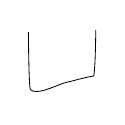
\begin{tikzpicture}[x={\dimexpr\dimen0/1180\relax},y={\dimexpr-\dimen2/335\relax},line width=.3pt]
\path[use as bounding box] (0,0) rectangle (1180,335);
\draw (12,22) .. controls (16,107) and (21,271) .. (45,301) .. controls (145,328) and (405,292) .. (602,271) .. controls (784,258) and (1020,239) .. (1133,235) .. controls (1155,199) and (1164,88) .. (1167,12);
\end{tikzpicture}}}%
\kern\dimen4\box0\kern\dimen8\endgroup}

\mspage{-0.27-}

\uline{Proposition} \uline{0.9}: Let $S=\operatorname{Spec}(k)$, $k$ a field, and assume that
\begingroup
\setbox0=\hbox{$G$,}
\dimen0=\wd0 \divide\dimen0 by 37 \multiply\dimen0 by 110
\dimen2=\ht0 \advance\dimen2 by \dp0 \divide\dimen2 by 27 \multiply\dimen2 by 115
\dimen4=\dimen0 \divide\dimen4 by 110 \multiply\dimen4 by 50
\dimen6=\dimen2 \divide\dimen6 by 115 \multiply\dimen6 by 30
\dimen8=\dimen0 \advance\dimen8 by -\wd0 \advance\dimen8 by -\dimen4
\leavevmode\rlap{\raisebox{\dimexpr-\dp0-\dimen6\relax}{%
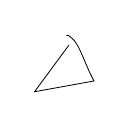
\begin{tikzpicture}[x={\dimexpr\dimen0/110\relax},y={\dimexpr-\dimen2/115\relax},line width=.3pt]
\path[use as bounding box] (0,0) rectangle (110,115);
\draw (66,29) -- (11,107) -- (106,89) .. controls (92,63) and (82,25) .. (70,17) .. controls (67,13) and (63,12) .. (62,13);
\end{tikzpicture}}}%
\kern\dimen4\box0\kern\dimen8\endgroup
$X$ and $Y$ are algebraic schemes over $k$. If the action $\sigma$ is
\begingroup
\setbox0=\hbox{free,}
\dimen0=\wd0 \divide\dimen0 by 50 \multiply\dimen0 by 110
\dimen2=\ht0 \advance\dimen2 by \dp0 \divide\dimen2 by 35 \multiply\dimen2 by 95
\dimen4=\dimen0 \divide\dimen4 by 110 \multiply\dimen4 by 30
\dimen6=\dimen2 \divide\dimen6 by 95 \multiply\dimen6 by 30
\dimen8=\dimen0 \advance\dimen8 by -\wd0 \advance\dimen8 by -\dimen4
\leavevmode\rlap{\raisebox{\dimexpr-\dp0-\dimen6\relax}{%
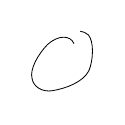
\begin{tikzpicture}[x={\dimexpr\dimen0/110\relax},y={\dimexpr-\dimen2/95\relax},line width=.3pt]
\path[use as bounding box] (0,0) rectangle (110,95);
\draw (74,22) .. controls (68,10) and (49,10) .. (32,23) .. controls (16,37) and (3,58) .. (7,70) .. controls (9,82) and (24,89) .. (39,87) .. controls (61,84) and (89,75) .. (98,59) .. controls (105,44) and (106,19) .. (97,10) .. controls (93,7) and (88,5) .. (84,5);
\end{tikzpicture}}}%
\kern\dimen4\box0\kern\dimen8\endgroup
and $(Y,\phi)$ is a geometric quotient of $X$ by $G$, then $X$ is a principal fibre bundle over $Y$ with group $G$.\({}^*\)

\margin{\figure{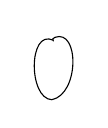
\begin{tikzpicture}[x=1em,y=1ex]
\draw (.05,2.55) .. controls (-.85,3.5) and (-.85,-2.35) .. (0,-2.45)
.. controls (1.0,-2.0) and (1.0,3.55) .. (.11,2.78)
.. controls (.05,2.72) and (.00,2.61) .. (.06,2.45);
\end{tikzpicture}}\unsure{large} seem enough?}

\margin{\figure{
\begin{tikzpicture}[baseline=-.5ex,x=.028em,y=-.038ex]
\draw (9,0) -- (39,25) -- (0,69) .. controls (2,45) and (6,20) .. (9,0);
\end{tikzpicture}}$G$ \uline{smooth}$/k$!}

\uline{Proof}: First of all, we may assume that $k$ is algebraically closed: for by such a base extension, i) $\sigma$ remains free, ii) $(Y,\phi)$ remains a geometric quotient (Remark $\unsure{7|\gamma}$, \S2), iii) the property of being a principal fibre bundle descends (SGA 8, 5.4). Secondly, we may replace $Y$ by one of its local rings $\operatorname{Spec}(\underline{o}_{y,Y})$, for some closed point $y\in Y$: for all conditions of Definition 0.10 are expressible locally. And thirdly, we may replace $\operatorname{Spec}(\underline{o}_{y,Y})$ by $\operatorname{Spec}(\hat{\underline{o}}_{y,Y})$ (its completion). For this is also a faithfully flat quasi-compact base extension and, as before, i) $\sigma$ remains free, ii) $(Y,\phi)$ remains a geometric quotient, and iii) the property of being a principal fibre bundle descends.

Therefore we have $Y=\operatorname{Spec}(A)$, where $A$ is a complete local ring with algebraically closed residue field. Let $y$ be the closed point of $Y$, and let $x$ be a closed, hence $k$-rational point of $X$ over $y$. Let $I_x\subset\underline{o}_{x,X}$ be
\begingroup
\setbox0=\hbox{the}
\dimen0=\wd0 \divide\dimen0 by 31 \multiply\dimen0 by 78
\dimen2=\ht0 \advance\dimen2 by \dp0 \divide\dimen2 by 27 \multiply\dimen2 by 108
\dimen4=\dimen0 \divide\dimen4 by 78 \multiply\dimen4 by 22
\dimen6=\dimen2 \divide\dimen6 by 108 \multiply\dimen6 by 38
\dimen8=\dimen0 \advance\dimen8 by -\wd0 \advance\dimen8 by -\dimen4
\leavevmode\rlap{\raisebox{\dimexpr-\dp0-\dimen6\relax}{%

\begin{tikzpicture}[x={\dimexpr\dimen0/78\relax},y={\dimexpr-\dimen2/108\relax},line width=.3pt]
\path[use as bounding box] (0,0) rectangle (78,108);
\draw (38,23) .. controls (42,8) and (34,17) .. (27,29) .. controls (17,44) and (6,62) .. (6,82) .. controls (6,98) and (20,102) .. (34,96) .. controls (54,86) and (69,72) .. (70,48) .. controls (72,34) and (61,20) .. (55,22) .. controls (51,23) and (51,27) .. (51,29);
\end{tikzpicture}}}%
\kern\dimen4\box0\kern\dimen8\endgroup
ideal defining
\begingroup
\setbox0=\hbox{the orbit $O(x)$}
\dimen0=\wd0 \divide\dimen0 by 210 \multiply\dimen0 by 295
\dimen2=\ht0 \advance\dimen2 by \dp0 \divide\dimen2 by 35 \multiply\dimen2 by 100
\dimen4=\dimen0 \divide\dimen4 by 295 \multiply\dimen4 by 40
\dimen6=\dimen2 \divide\dimen6 by 100 \multiply\dimen6 by 35
\dimen8=\dimen0 \advance\dimen8 by -\wd0 \advance\dimen8 by -\dimen4
\leavevmode\rlap{\raisebox{\dimexpr-\dp0-\dimen6\relax}{%
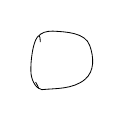
\begin{tikzpicture}[x={\dimexpr\dimen0/295\relax},y={\dimexpr-\dimen2/100\relax},line width=.3pt]
\path[use as bounding box] (0,0) rectangle (295,100);
\draw (54,21) .. controls (53,8) and (47,11) .. (39,15) .. controls (24,22) and (11,47) .. (14,66) .. controls (18,79) and (39,89) .. (61,90) .. controls (116,88) and (193,90) .. (246,75) .. controls (287,63) and (284,43) .. (266,26) .. controls (247,7) and (164,6) .. (107,5) .. controls (79,5) and (59,7) .. (44,13);
\draw (34,79) .. controls (41,82) and (44,86) .. (47,88);
\end{tikzpicture}}}%
\kern\dimen4\box0\kern\dimen8\endgroup
of $x$. Since $\sigma$ is free, the morphism $\psi_x$ defines an isomorphism:

\[
\underline{o}_{x,X}/I_x\xrightarrow{\sim}\underline{o}_{e,G}.
\]

\margin{ambiguous}

\noindent\rule{2cm}{.4pt}

\({}^*\)It seems very likely that this result holds even if we do not assume \uline{a} \uline{priori} that $Y$ is an algebraic scheme; and that it then follows \uline{a} \uline{posteriori} that $Y$ is an algebraic scheme.

\margin{\rotatebox{180}{56}}
